\chapter{链路估计器}\label{le}

\section{简介}
  链路估计器主要用于估计节点间的链路质量,以供路由引擎计算路由。
  TinyOS 2.x中实现的链路估计器结合了广播LEEP帧的收发成功率和单播数据包的
  发送成功率来计算单跳双向链路质量。

  链路估计器的实现是多样化的,但是必须遵循TEP 124\ucite{tep124}中的协议规范。使用网络各层中不同
  的信息可以得到不同的估计结果,各种方法都有其长处和缺点。在下面“实现”一节中我们将
  分析3种TinyOS中自带的实现。

\section{基本概念}
  \subsection{LEEP协议}
	链路估计交换协议(Link Estimation Exchange Protocol,LEEP)用于在
	节点间交换链路估计信息,定义了交换信息使用的LEEP帧的详细格式。
  \subsection{入站链路质量}
	如图\ref{fig:subfig:a}所示,有节点对$(A,B)$,以B作为参考节点,A向B发送的总帧数为
    $total_{in}$,其中B成功接收到的帧数为$success_{in}$,从而有:
	\begin{equation}
		\text{\kai 入站链路质量} = \frac{success_{in}}{total_{in}}
	\end{equation}

    $total_{in}$的值可以通过A节点
    广播的LEEP帧中的顺序号间接计算而得。LEEP帧中设有顺序号字段,节点A每
    广播一次LEEP帧,它会将该字段加1,B节点只需要计算连续收到的LEEP帧
    顺序号的差值就可以得到A总共发送的LEEP帧数。

    入站链路质量也可以通过其它途径得到,比如LQI或RSSI之类的链路质量指示
    器,不过这需要无线模块支持这类功能才行。
\begin{figure}[ht]
\centering
\subfigure[入站链路质量]{
\label{fig:subfig:a}
\begin{minipage}[b]{0.2\textwidth}
\centering
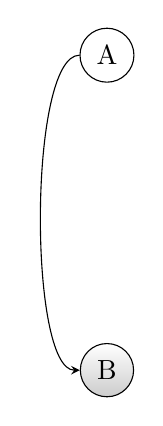
\begin{tikzpicture}[>=stealth]
	\node[circle,draw]  (A) at (0,4) {A};
	\node[circle,draw,top color=white,bottom color=black!20]  (B) at (0,0) {B};

	\draw[->] (A)  .. controls +(left:1) and +(left:1) ..  (B);
\end{tikzpicture}
\end{minipage}}
\hspace{1cm}
\subfigure[出站链路质量]{
\label{fig:subfig:b}
\begin{minipage}[b]{0.2\textwidth}
\centering
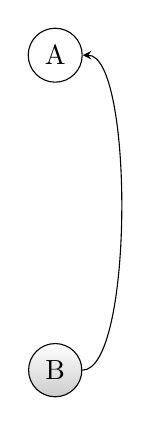
\begin{tikzpicture}[>=stealth]
	\node[circle,draw]  (A) at (0,4) {A};
	\node[circle,draw,top color=white,bottom color=black!20]  (B) at (0,0) {B};

	\draw[->] (B)  .. controls +(right:1) and +(right:1) ..  (A);
\end{tikzpicture}
\end{minipage}}
\hspace{1cm}
\subfigure[双向链路质量]{
\label{fig:subfig:c}
\begin{minipage}[b]{0.2\textwidth}
\centering
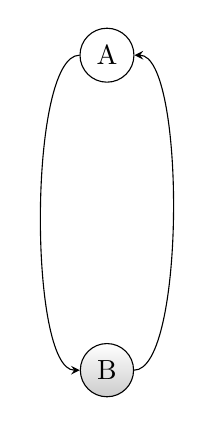
\begin{tikzpicture}[>=stealth]
	\node[circle,draw]  (A) at (0,4) {A};
	\node[circle,draw,top color=white,bottom color=black!20]  (B) at (0,0) {B};

	\draw[->] (A)  .. controls +(left:1) and +(left:1) ..  (B);
	\draw[->] (B)  .. controls +(right:1) and +(right:1) ..  (A);
\end{tikzpicture}
\end{minipage}}
\caption{三种链路质量}\label{link-quality}
\end{figure}


  \subsection{出站链路质量}
    如图\ref{fig:subfig:b}所示,节点对$(A,B)$,以B作为参考点,B向A发送帧数为$total_{out}$,
    其中A成功接收到帧数为$success_{out}$,从而有:
	\begin{equation}
		\text{\kai 出站链路质量} = \frac{success_{out}}{total_{out}}
	\end{equation}

    由于LEEP帧是通过广播方式发送的,节点B无法得知节点A是否收到,从而
    无法计算$success_{out}$。但B到A的出站链路质量即A到B的入站链路质量,要解决
    该问题只有让A把它与B间的入站链路质量回馈给B,这其实就是LEEP帧的主要
    功能之一。

    TinyOS 2.x中用8位无符号整数表示出站或入站链路质量。为了减少精度损失和
    充分利用8位的空间,TinyOS 2.x在实际存储该值时对它扩大255倍。

  \subsection{双向链路质量}
    如图\ref{fig:subfig:c}所示,对于有向节点对$(A,B)$,双向链路质量定义如下:
	\begin{equation}
		\text{\kai 双向链路质量} = \text{\kai 入站链路质量} \times \text{\kai 出站链路质量}
	\end{equation}

    本地干扰或噪声可以引起$(A,B)$和$(B,A)$链路质量不同,定义双向链路质量
    就是为了将这种情况考虑在内。
  \subsection{EETX值}
    TinyOS 2.x中使用EETX(Extra Expected number of Transmission)值表示双向链路质量估计值。
    在LEEP协议中使用的有两种EETX值:{\kai 窗口EETX}和{\kai 累积EETX}。窗口EETX是接收到的LEEP帧数或发送
    的数据包数达到一个固定的窗口大小时,根据窗口中的收发成功率计算出的EETX。而累积EETX则
    是本次窗口EETX和上次累积EETX加权相加得到的。根据指数移动平均的原理让旧值的权重逐渐减少,
    以适应链路质量的变化,是比较符合实际的统计方法。

\section{LEEP协议对数据链路层的要求}
\noindent LEEP协议对数据链路层有以下三个要求:
\vspace{-8pt}
\begin{enumerate}
	\item 有单跳源地址
	\item 提供广播地址
	\item 提供LEEP帧长度
\end{enumerate}
\vspace{-8pt}

  其中,有单跳源地址的要求是为了让收到广播LEEP帧的节点确定更新邻居表中哪一项
  的出站链路质量。现有节点的数据链路层一般都可以满足这3个要求。

\section{LEEP帧结构}
  根据以上分析可以得知LEEP帧至少应具备一个顺序号和与邻居节点间的入站链路质量。
  TinyOS 2.x中实现的LEEP帧结构如图\ref{leep-frame-structure}所示:
\begin{figure}[ht]
\centering
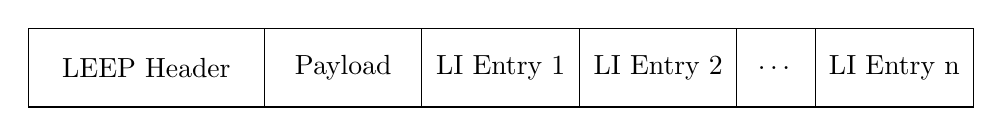
\begin{tikzpicture}
	\pagella
	\draw (0,0) rectangle (12,1);
	\foreach \x in {3,5,7,9,10,12}
	{
	  \draw (\x,0) -- (\x,1);
	}
	\foreach \x/\txt in {1.5/LEEP Header,4/Payload,6/LI Entry 1,8/LI Entry 2,9.5/\dots,11/LI Entry n}
	{
	  \draw (\x,0.5) node {\txt};
	}
\end{tikzpicture}
\caption{LEEP帧结构}\label{leep-frame-structure}
\end{figure}

  其中LEEP头部结构如图\ref{leep-frame-head}所示:

\begin{figure}[ht]
\centering
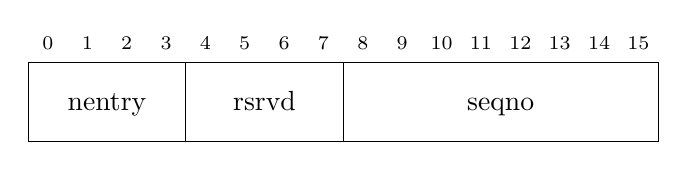
\begin{tikzpicture}
	\pagella
	\draw (0,0) rectangle (8,1);
	\foreach \x in {0,...,15}
	{
	  \draw (\x*0.5+0.25,1.25) node {\scriptsize \x};
	}
	\foreach \x in {2,4}
	{
	  \draw (\x,0) -- (\x,1);
	}
	\foreach \x/\txt in {1/nentry,3/rsrvd,6/seqno}
	{
	  \draw (\x,0.4) node[anchor=base] {\txt};
	}
\end{tikzpicture}
\caption{LEEP帧头部}\label{leep-frame-head}
\end{figure}

  各字段定义:
\vspace{-10pt}
\begin{itemize}
	\item nentry:尾部的LI项个数
	\item seqno:LEEP帧顺序号
	\item rsrvd:保留字段必须设为0
\end{itemize}
\vspace{-5pt}

    链路信息项格式如图\ref{link-info-frame}所示:

\begin{figure}[ht]
\centering
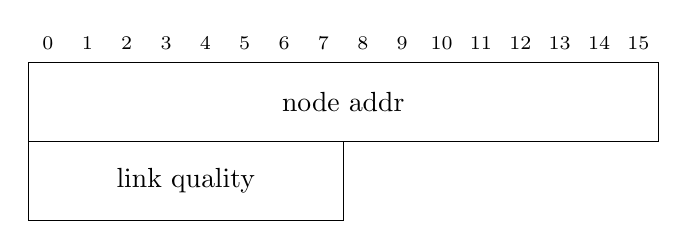
\begin{tikzpicture}
	\pagella
	\draw (0,0) rectangle (8,1);
	\foreach \x in {0,...,15}
	{
	  \draw (\x*0.5+0.25,1.25) node {\scriptsize \x};
	}
	\draw (4,0.5) node {node addr};
	\draw (0,0) -- (0,-1)--(4,-1)--(4,0);
	\draw (2,-0.5) node {link quality};
\end{tikzpicture}
\caption{链路信息项}\label{link-info-frame}
\end{figure}

    各字段定义如下:
\vspace{-10pt}
\begin{itemize}
	\item node addr:邻居节点的链路层地址
	\item link quality:从与node id对应的节点到本节点的入站链路质量
\end{itemize}

\section{实现}
  TinyOS中可选的链路估计器有两种:标准LE估计器和4位链路估计器。可以通过更改应用程序Makefile
中对应的路径选择使用哪一个链路估计器。
  \subsection{标准LE估计器}
  TinyOS 2.x中标准LE估计器的实现在\texttt{tos/lib/net/le}目录下:
\vspace{-10pt}
\begin{itemize}
  \item {\texttt{LinkEstimator.h}}:	头文件,包含了邻居表大小、邻居表项结构、LEEP帧头尾结构
  			以及LEEP协议中用到的常数的定义。
  \item {\texttt{LinkEstimator.nc}}:	接口定义。包含了其它组件可以从LinkEstimator中调用的方法。由如下代码所示,这些方法可以分三类,一类用于获取链路质量,一类用于操作邻居表,还有一类用于数据包估计。

%\begin{lstlisting}[captionpos=b,caption={LinkEstimator接口},label=linkestimator-h]
\begin{lstlisting}
interface LinkEstimator {
	command uint16_t getLinkQuality(uint16_t neighbor);
	command uint16_t getReverseQuality(uint16_t neighbor);
	command uint16_t getForwardQuality(uint16_t neighbor);

	command error_t insertNeighbor(am_addr_t neighbor);
	command error_t pinNeighbor(am_addr_t neighbor);
	command error_t unpinNeighbor(am_addr_t neighbor);

	command error_t txAck(am_addr_t neighbor);
	command error_t txNoAck(am_addr_t neighbor);
	command error_t clearDLQ(am_addr_t neighbor);

	event void evicted(am_addr_t neighbor);
}
\end{lstlisting}
  \item {\texttt{LinkEstimatorC.nc}}:	配置文件,用于说明链路估计器提供LinkEstimator接口。
  \item {\texttt{LinkEstimatorP.nc}}:	LEEP协议具体实现。
\end{itemize}
\vspace{-10pt}
  
    LEEP协议的目的是为了得到本节点到邻居节点间的双向链路质量。实现中使用两种策略
    相结合来计算估计值,两者间的关系如图\ref{ld-estimate}所示:
\begin{figure}[ht]
\centering
\begin{tikzpicture}[>=latex]
	\usetikzlibrary{shapes.multipart}
	\tikzstyle{rec}=[minimum width=1cm,minimum height=1cm,rectangle,draw]
	\draw (-1,6) node[text width=1.8cm,text centered] (A) {广播\\ EETX帧};
	\draw (-1,2) node[text width=2.8cm,text centered] (B) {转发引擎\\ACK接收情况};

	\node[rec] (WL) at (1.5,6) {窗口};
	\node[rec] (WD) at (1.5,2) {窗口};
	\node[rec] (L) at (3.5,6) {L估计};
	\node[rec] (D) at (3.5,2) {D估计};

	\node[rec] (EMA) at (5,4) {指数移动平均};
	\node[rec] (OEETX) at (7,1) {原EETX};
	\node[rec] (EETX) at (9,4) {累积EETX};

	\path (A) edge[->] (WL) ;
	\path (B) edge[->] (WD);
	\path (WL) edge[->] node[above]{\fontsize{9pt}{9pt}满} (L);
	\path (WD) edge[->] node[above]{\fontsize{9pt}{9pt}满} (D);
	\path (L) edge[->] (EMA);
	\path (D) edge[->] (EMA);
	\path (EMA) edge[->] (EETX);
	\path (EETX) edge[->] (OEETX);
	\path (OEETX) edge[->] (EMA);
	\node[rotate=56] at (8.3,2.4) {\fontsize{9pt}{9pt}下一次计算};
\end{tikzpicture}


\caption{链路估计值计算}\label{ld-estimate}
\end{figure}

    \subsubsection{根据LEEP帧的估计(L估计)}
      LEEP帧的估计通过LEEP帧的信息来估计EETX值。

      LEEP帧的发送:使用Send.send()方法,调用addLinkEstHeaderAndFooter()函数加LEEP
      	头尾。尾部存放的是本节点到邻居节点的链路质量表,如果LEEP帧中一次放不下
	这个表,则在下次发LEEP帧时从首个上次放不下的表项放起,以保证每个表项
	有平等的发送机会。每发一个包都将帧中的顺序号字段加1。
	发送的时机由LinkEstimator的使用者决定。

      LEEP帧的接收:每当收到一个LEEP帧,会触发SubReceive.receive()事件。
	处理程序根据LEEP头尾信息更新邻居表。这些操作集中在函数
      	processReceiveMessage()中进行,该函数找到这个LEEP帧发送者对应的邻居表项,调用
	updateNeighborEntryIdx()函数更新收到包数计数值和丢包数计数值。其中的丢包数就
	是本次与上次LEEP帧中顺序号字段的差值。

	当收到的包数达到一个固定窗口的大小时,
	调用updateNeighborTableEst()函数计算该窗口中的入站链路质量~$inquality_{win}$:
	\begin{equation}
      		inquality_{win} = 255 \times \frac{\text{\kai 接收到LEEP帧数}}{\text{\kai 总帧数}}
	\end{equation}
        根据动态移动平均原理更新入站链路质量:
	\begin{equation}
		inquality = \frac{\alpha \times inquality_{orig} + (10 - \alpha) \times inquality_{win}} {10}
	\end{equation}
	  TinyOS 2.x中设衰减系数$\alpha$值为9,因此每次更新时,旧值占$\frac{9}{10}$的权重,而新
	  值占$\frac{1}{10}$的权重。

	入站链路质量发生了变化,因此需要相应地计算双向链路质量。首先计算窗口EETX值~$EETX_{win}$:
	\begin{equation}
		EETX_{win} = (\frac{255^2}{inquality \times outquality} - 1) \times 10
	\end{equation}
	为了提高存储精度,EETX值都是扩大10倍存储。

	接着更新累积EETX值:
	\begin{equation}
		EETX = \frac{\alpha \times EETX_{orig} + (10-\alpha) \times EETX_{win}}{10}
	\end{equation}

    \subsubsection{根据数据包的估计(D估计)}
      根据数据包的估计通过发送数据包的成功率来估计EETX值。

      LinkEstimator并不能得知上层的数据包是否发送成功。因此它提供两个命令txAck()和txNoAck()
      让上层组件调用。txAck()用于告知链路估计器数据包发送成功,它将对应通信邻居的成功传输
      数据包计数值和总传输包计数值加1。当总传输包数达到一个固定窗口的大小时,调用updateDEETX()
      函数计算窗口EETX值~$DEETX_{win}$:
	\begin{equation}
      		DEETX_{win} = (\frac{\text{\kai 总包数}}{\text{\kai 成功包数}} - 1) \times 10
	\end{equation}
      接着更新累积EETX值:
	\begin{equation}
      		EETX = \frac{\alpha \times EETX_{orig} + (10-\alpha) \times DEETX_{win}}{10}
	\end{equation}

\subsection{四位链路估计(4BITLE)}
四位链路估计\ucite{fonseca2007fbw}与标准LE估计器的实现在结构上大体上是相同的。有所改进的是它提炼了物理层、链路层和网络层回馈的信息用于更精确的链路估计。其中1位来自物理层,1位来自链路层,2位来自网络层。4BITLE的实现在\texttt{tos/lib/net/4bitle}目录下。

\subsubsection{物理层}
在物理层,我们可以从一个包的传输中测量信道的质量。通常情况下,接收到错误位比较少的包很可能比错误多的包链路质量好。物理层的测量是快速并且廉价的,可以避免估计器在网络边缘或劣质的连接上浪费精力。我们可以把它提炼为一个white位,它表示在接收包时信道链路质量的优劣程度。

\subsubsection{链路层}
在链路层,我们可以测量包是否被传输并确认。基于广播探测的估计器面临着一个问题,它们将链路估计和数据通信分开实现,如果链路质量变坏导致包丢失,链路估计器要直到下一个路由信标被丢弃时才能反映这种变化。为了解决该问题,我们使用一个ack位,表示节点在一次传输中是否收到链路层的确认。

\subsubsection{网络层}
在网络层,我们可以了解到哪个连接是高层性能上最有价值的。如果没有网络层的信息,估计器可能选择一条路由环路,或者在最坏的情况下会与网络失去连接。无线传感器网络很可能会因链路层和网络层链路表的不一致而导致故障。我们可把这些提炼为2个位:
\vspace{-10pt}
  \begin{itemize}
	\item{pin位:} 用于告诉估计器不能剔除正在使用的连接。
	\item{compare位:} 用于告诉网络层这个连接看起来颇有希望。
  \end{itemize}

\subsection{链接质量指示(LQI)}
链接质量指示(Link Quality Indicator, LQI)是MultiHopLQI汇聚协议中用于链路估计的部分。它需要无线模块支持LQI,因此它只适用于CC2420之类具有链接质量指示器的节点。它完全使用物理层的信息作链路估计。
